\begin{enumerate}[label=\thesubsection.\arabic*.,ref=\thesubsection.\theenumi]
\numberwithin{equation}{enumi}


\item The asymptotic Bode phase plot of 
%
\begin{align}
\label{eq:ee18btech11037_gs}
G(s) = \frac{k}{(s+0.1)(s+10)(s+{p_1})}
\end{align}
%
with k and $p_1$ both positive, is shown below.
\begin{figure}[!ht]
\centering
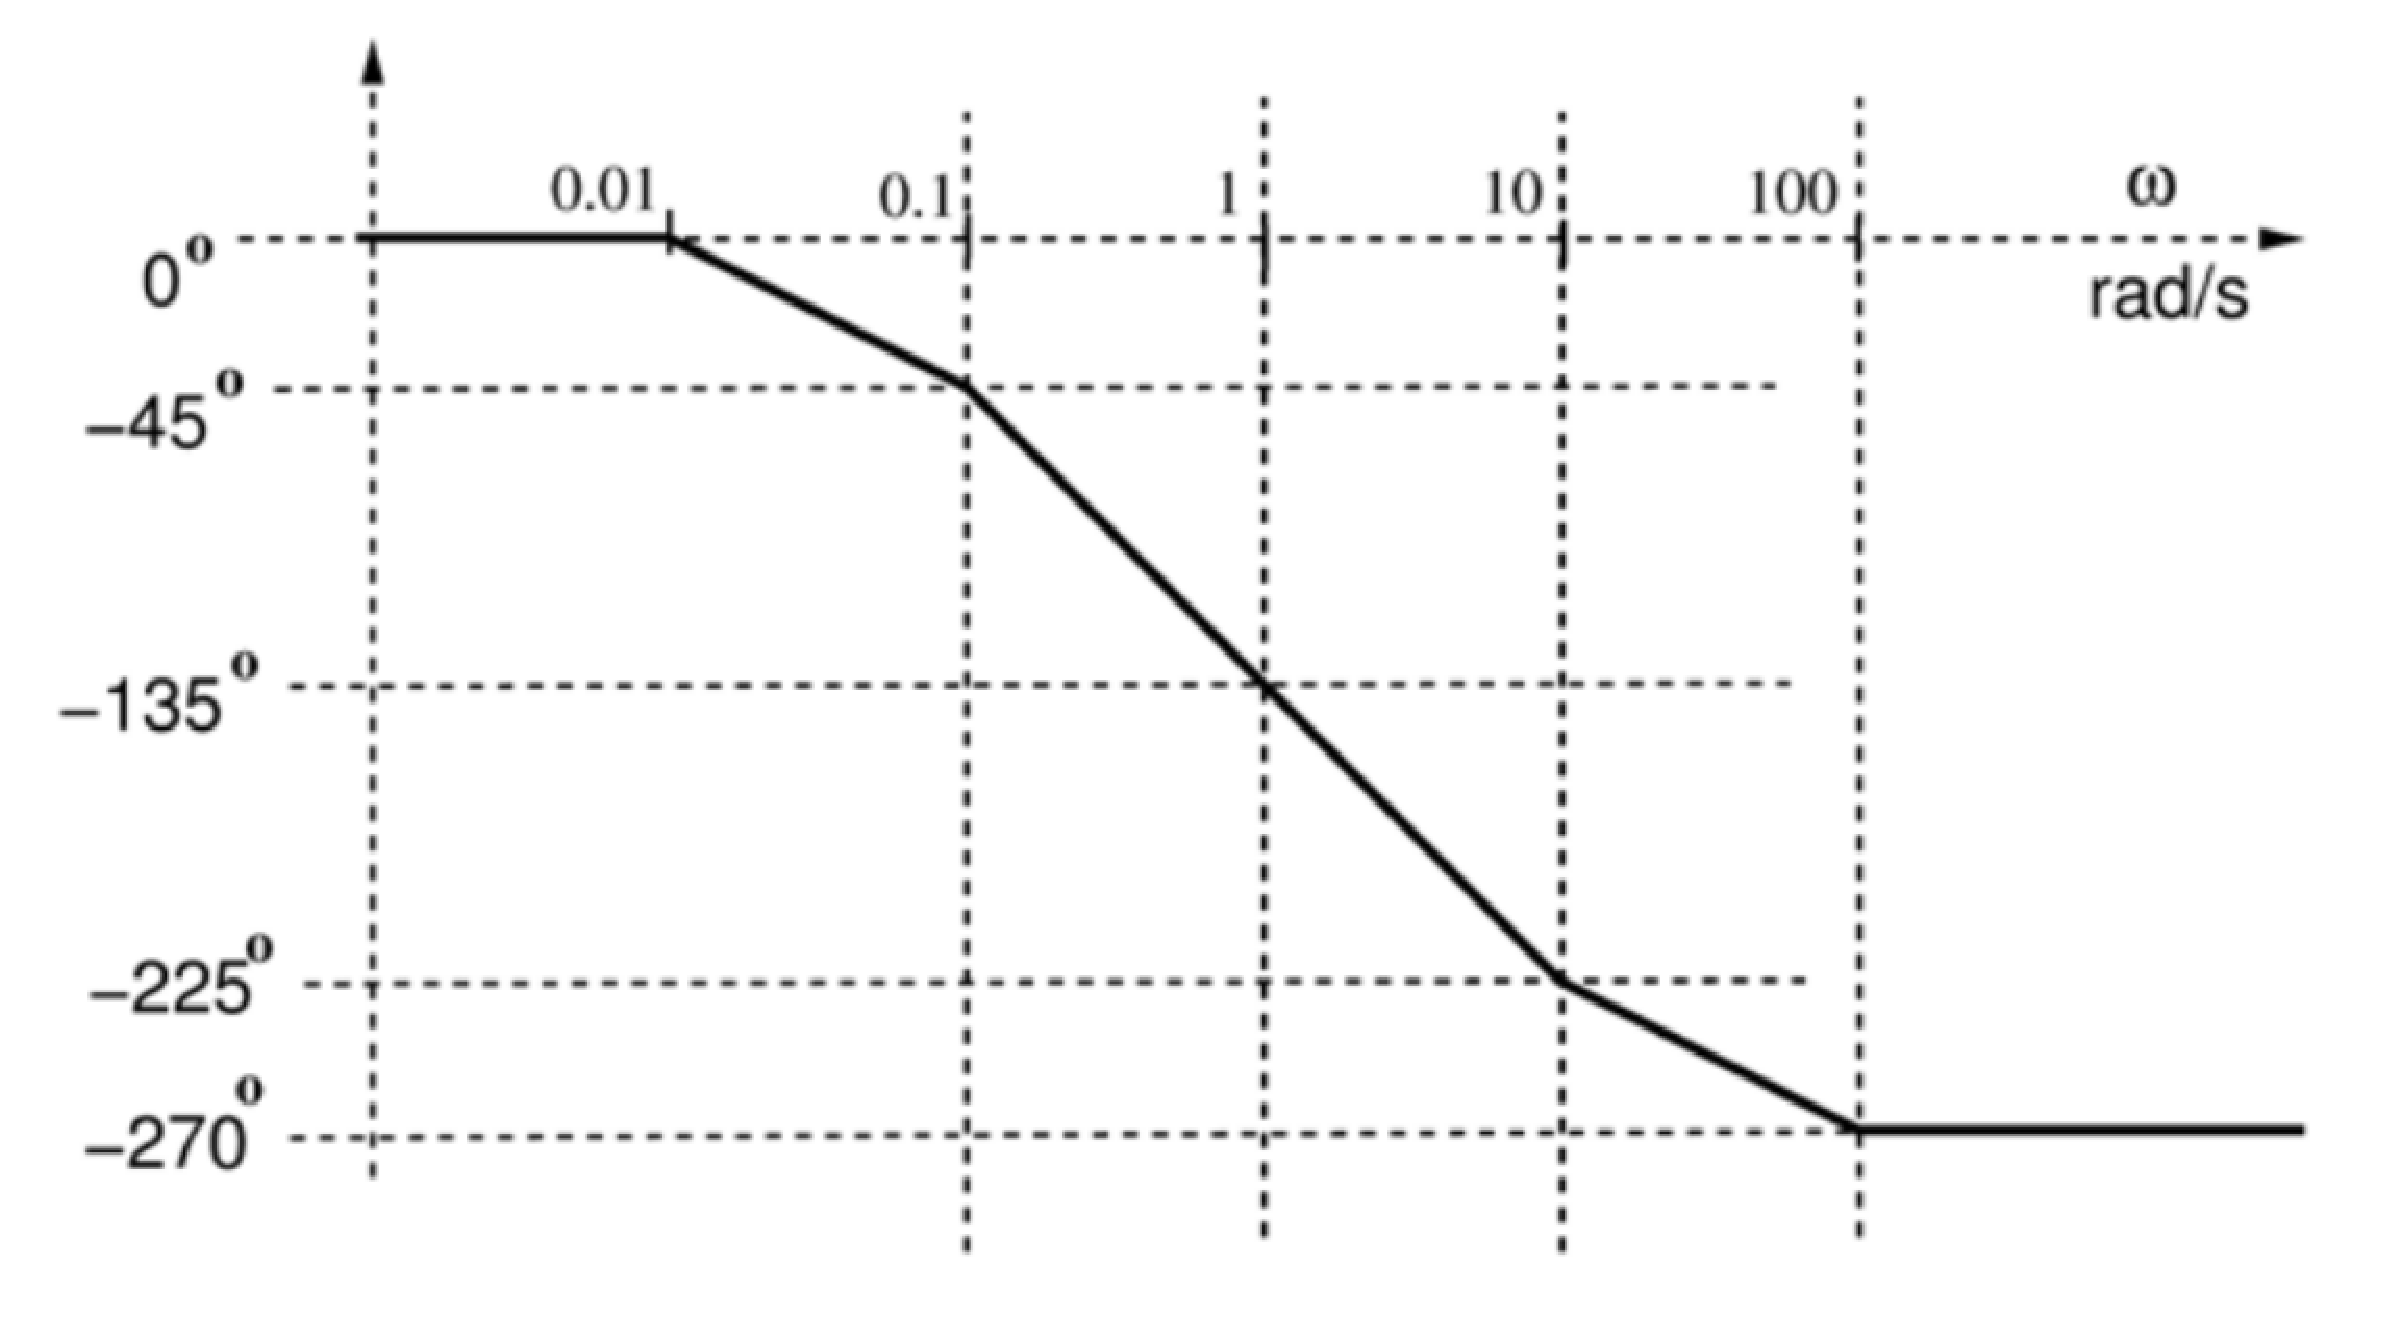
\includegraphics[width=\columnwidth]{figs/ee18btech11037/ee18btech11037.eps}
\caption{}
\label{fig:ee18btech11037}
\end{figure}
Find the value of \textit{$p_1$}.
\\
\solution
Phase of this transfer function,
\begin{align}
\phi(\omega) = -\tan^{-1} \brak{\frac{\omega}{0.1}}-\tan^{-1} \brak{\frac{\omega}{10}}-\tan^{-1} \brak{\frac{\omega}{p_1}}
\end{align}
From the plot,
\begin{align}
-45\degree = -\tan^{-1}\brak{\frac{0.1}{0.1}} -\tan^{-1}\brak{\frac{0.1}{10}} -\tan^{-1}\brak{\frac{0.1}{p_1}}
\end{align}
 $p_1$ is approximately 1, i.e, for $p_1$ in 0.95 to 1.05 the $\phi$ is approximately equals to $-45\degree$.
%
\item Find the value of $p_1$ using bode phase plot properties.
\\
\solution In asymptotic Bode plot for a single pole, the phase at pole is $-45\degree$ and the phase changes from 0 to -90 in 2 decades i.e, from $pole/10$ to $10\times pole$.
\\
Bode phase plot for a transfer function having pole at p
\begin{align}
 \phi(\omega) = 
 \begin{cases} 
        0 & 0<f< p/10 \\
      -45\times\brak{\log(f)-\log(p/10)}& p/10<f<10p \\
      -90 & 10p<f  
 \end{cases}
\end{align}
\\
Adding the bode phase plots corresponding to the 0.1,10.
\begin{figure}[!ht]
\centering
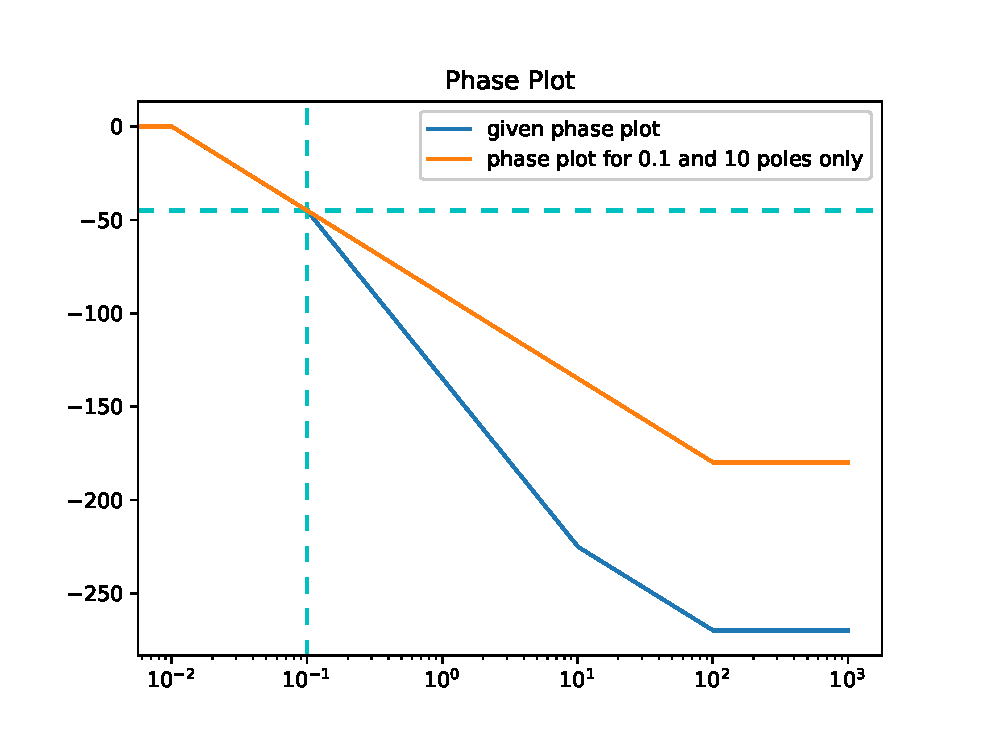
\includegraphics[width=\columnwidth]{figs/ee18btech11037/ee18btech11037_2.eps}
\caption{}
\label{fig:ee18btech11037_2}
\end{figure}
\\
The values before the 0.1 does not change when compared to figure \ref{fig:ee18btech11037}, so $p_1/10$ is greater than or equal to 0.1.
\\
In the plot obtained by adding these two plots the slope at 0.1 doesnt change, but in figure \ref{fig:ee18btech11037} there is a change so $p/10 = 0.1 $ 
\begin{align}
\implies p_1 = 1
\end{align}
The following code plots Fig. \ref{fig:ee18btech11037_2}

\begin{lstlisting}
codes/ee18btech11037.py
\end{lstlisting}

\end{enumerate}
